\chapter{On the dynamics of acyl carrier protein}
\label{cha:chap5}

\section{Introduction}
\label{sec:chap5-Intro}
Acyl carrier proteins play an important role in shuttling substrates and products in fatty acid and polyketide biosynthesis. Inspite of being expressed in a minuscule amount (e.g. $ \approx $0.25\% of all the soluble proteins in an \textit{E. coli} cell), the dynamic nature of these proteins helps them to interact with several different core and auxiliary domains in the FAS and PKS machinery. An ACP is a four helix bundle with three helices I, II and IV running parallel to each other, while helix III runs perpendicular to the others. A holo ACP is an ACP charged with phosphopantetheine, a prosthetic linker derived from coenzyme A, which is transferred to the ACP  by ACP synthases. The Holo ACP then tethers an acyl group to the terminal sulfhydryl of its phosphopantetheine via a thioester linkage. Experiments and molecular dynamics studies on FAS ACPs have shown the sequestering of acyl substrates within the hydrophobic core formed by the four helix bundle. However, it is not known if there is a similar mechanism in PKS ACPs. 

\textcite{Chan2008} conducted molecular dynamics simulations on apo, holo, and acyl forms of \textit{E. coli} FAS ACP which suggested a mechanism for acyl chain binding inside the ACP core. Simulations were performed using an experimentally determined holo FAS ACP structure (PDB ID 1L0I) with a butyryl molecule trapped inside the core of a holo ACP. Several different lengths of acyl chain were constructed by extending the butyryl molecule by two carbons at a time up to eighteen carbons. Simulations were conducted starting with the acyl chains in solvent exposed as well as in buried states and solvent exposed acyl chains up to ten carbons long easily found their way into the hydrophobic core of the ACP, stably residing in the core till the end of a 50 ns simulation. However, longer acyl chains found it difficult to find there way into the ACP core, and were not consistently stable in the core till the end of simulations. \textcite{Chan2008} proposed an eight carbon acyl chain as the optimal for stable accommodation by this FAS ACP (PDB ID 1L0I). They also found a novel binding pocket in which the acyl chain was directed towards helix I as opposed to the binding pocket in the solved structure. Simulations also highlighted residues T39 and E60 as stabilizing the position of the phosphopantetheine linker through hydrogen bonds at the opening of the hydrophobic tunnel. 

Here, molecular dynamics (MD) simulations of the apo, holo, and acyl forms of ACP-mupA3a and the acyl form of ACP-mupA2a from the mupirocin cluster are presented in order to investigate the dynamic behaviour of the PKS ACPs upon phosphopantetheine and acyl chain attachment. The main property of interest was to detect the formation of a cavity or tunnel that could sequester a PKS substrate, similar to that seen in the FAS ACP. MD simulation trajectories were analysed to calculate the hydrogen bonds formed by the phosphopantetheine and by the substrates, in the holo and acyl forms respectively, with the protein surface and the solvent. MD trajectories were also analysed to calculate the solvent accessible surface area (SASA) of the phosphopantetheine and the substrates in the holo and acyl forms respectively. %A correlation was calculate between the change in the number of hydrogen bonds and the change in the cavity volume during the simulations. 
To test whether the PKS ACPs become more like FAS ACPs in their holo and acyl forms, root mean square deviations (RMSD) of the PKS ACPs from the reference FAS ACP (PDB ID 1LOI) were calculated. %A corrleation was also calculated between the change in the RSMD and the change in the cavity volume during the simulations.    %Molecular dynamics simulations of the apo, holo, and acyl forms of ACP-mupA3a and the acyl form of ACP-mupA2a For ACP-mupA3a both the NMR determined structure of the wild type as well as a model of the W44L mutant were simulated in their apo, holo and acyl forms. For ACP-mupA2a a wild type modelled structure in the acyl form was used. Acyl forms of ACP-mupA3a and its W44L mutant were charged with unbranched monic acid and a fourteen carbon fully saturated carbon chain (mimicking the monic acid backbone). The acyl form of ACP-mupA2a was charged with a fourteen carbon mupirocin intermediate. Three independent simulations were run for 50 ns each for all the structures and one of the three simulations that showed a transition into the binding mode for holo and acyl forms was extended to 200 ns. One simulation for the wild type ACP-mupA3a charged with the unbranched monic acid was extended to 1 $ \mu $s.

\section{Results}
\label{sec:Chap5Results}

	\subsection{Molecular dynamics simulation setup and parameter determination}
	\label{sec:simSetup}
	In order to carry out molecular dynamics simulations of the apo, holo, and acyl forms of ACP-mupA3a and the acyl form of ACP-mupA2a, the first step was to generate the starting structures and assign the force field parameters. 
	
	For ACP-mupA3a two structures were used, a wild type (WT) and a W44L mutant. For the apo ACP-mupA3a WT, the NMR determined structure (PDB ID 2L22) was used as the starting conformation. For the apo ACP-mupA3a W44L, the same ACP-mupA3a structure was used but with the point mutation created by PyMol. To create the holo ACP structures, the catalytic S38 of their respective apo structures was extended with a phosphopantetheine. Two acyl forms of ACP-mupA3a WT were created, the first structure consists of the cognate substrate of the ACP-mupA3a (as shown in Figure \ref{fig:cognateSubstrates}) built directly onto the phosphopantetheine and was referred to as \textquotedblleft Acyl ACP-mupA3a WT\textquotedblright. The second acyl form consists of a fourteen carbon saturated chain built directly onto the phosphopantetheine of the holo ACP-mupA3a WT and was referred to as \textquotedblleft Acyl 14C ACP-mupA3a\textquotedblright. One acyl form of ACP-mupA3a W44L was also created by extending the phosphopantetheine of the holo ACP-mupA3a W44L with the cognate substrate of ACP-mupA3a and was referred to as \textquotedblleft Acyl ACP-mupA3a W44L\textquotedblright.
	 
	For ACP-mupA2a, as there was no experimentally determined structure available, a homology model was generated using as the template the ACP (PDB ID 2LIU) from the CurA module of the curacin system in \textit{Lyngbya Majuscula} (as described in Section \ref{sec:ACP2modelling}). To create the acyl form of ACP-mupA2 the catalytic serine of the modelled structure was extended with the phosphopantetheine followed by its cognate substrate (as shown in Figure \ref{fig:cognateSubstrates}) and was referred to as \textquotedblleft Acyl ACP-mupA2\textquotedblright. 

		\setlength\fboxsep{5pt}
		\setlength\fboxrule{1.5pt}
		\begin{figure}[htbp]
		\centering
		\fbox{\includegraphics[width=0.5\textwidth, keepaspectratio=true]{graphics/cognateSubstrates.pdf}}
		\caption[Cognate substrates for ACP-mupA2 and ACP-mupA3a in the mupirocin pathway.]{Cognate substrates for ACP-mupA2 and ACP-mupA3a in the mupirocin pathway.}
		\label{fig:cognateSubstrates}
		\end{figure}		
	
	Following the structure preparation the force field parameters were assigned to the atoms. Parameters from the AMBER99SB-ILDN force field were used for the protein atoms and GAFF parameters were used for the phosphopantetheine and the acyl chains with charges calculated using the RED server \parencite{Vanquelef2011}. A detailed description of the molecular dynamics simulations protocol and the procedure used to determine the parameters for the ligands is given in Section \ref{sec:MolecularDynamicSimulation} and Section \ref{sec:MDparameters} respectively.
	
	Multiple independent simulations were carried out for 50 ns for each of the holo and acyl forms, and one of the simulations that showed a transition into the binding mode was extended to 200 ns. One simulation for the Acyl ACP-mupA3a WT was further extended to 1 $ \mu $s. Simulation for the apo ACP-mupA3a WT was also extended to 1 $ \mu $s as a control. Table \ref{tab:simulationSetupSummary} summarizes the different simulations setup with reference to the methods sections for details. 
	
	\begin{table}[htbp]
	\caption{ACP simulation setup summary}
	\begin{tabularx}{\textwidth}{XXp{2cm}p{2cm}}
	\toprule[2pt]	
	\textbf{Structure} & \textbf{Ligand} &\textbf{Simulation} & \textbf{Method Section } \\
	\midrule[1pt]
	Apo ACP-mupA3a WT & -  & 1 X 1 $\mu$s & \ref{sec:WtoL_MD} B\\[5pt] 
	Apo ACP-mupA3a W44L & - & 1 X 200 ns & \ref{sec:WtoL_MD} B\\[5pt] 
	Holo ACP-mupA3a WT & phosphopantetheine & 4 X 50 ns  \newline 1 X 200 ns & \ref{sec:SPTsimulation}\\[5pt] 
	Holo ACP-mupA3a W44L & phosphopantetheine & 4 X 50 ns  \newline 1 X 200 ns & \ref{sec:SPTsimulation}\\[3pt] 
	Acyl ACP-mupA3a WT & ACP-mupA3a cognate substrate & 4 X 50 ns \newline 1 X 1 $\mu$s & \ref{sec:SPMsimulation} \\[5pt] 
	Acyl ACP-mupA3a W44L & ACP-mupA3a cognate substrate  & 4 X 50 ns \newline 1 X 200 ns & \ref{sec:SPMsimulation} \\[5pt] 
	Acyl 14C ACP-mupA3a & fourteen carbon saturated chain& 2 X 50 ns \newline 1 X 200 ns & \ref{sec:SPCsimulation} \\[5pt] 
	Acyl ACP-mupA2 & ACP-mupA2 cognate substrate & 2 X 50 ns \newline 1 X 200 ns &  \ref{sec:SPBsimulation}  \\
	\bottomrule[2pt]
	\end{tabularx}
	\label{tab:simulationSetupSummary}
	\end{table}
	
	
	\subsection{ACP backbone dynamics over time}
	\label{sec:backbonedynamics}
	All the simulations were stable, as indicated by the RMSD and RMSF calculations. The RMSD values of the backbone atoms from the reference starting structures remained below 2.5 \AA \ for all the simulations and plateaued within the first 50 ns. The root mean square fluctuation (RMSF) \nomenclature{RMSF}{Root mean square fluctuation} calculated for the backbone atoms, averaged per residue (as described in Section \ref{sec:RMSDstartingStructure}), showed a higher fluctuation in the mutant structures as compared to the wild type. This observation is consistent with the MD simulations mentioned in the Chapter 3, Section \ref{sec:WtoLMD}. However, upon attaching the cognate substrate of ACP-mupA3a, 200 ns and $ \mu $s simulations of the acyl ACP-mupA3a WT showed more fluctuation than the 200 ns simulations of acyl ACP-mupA3a W44L (Figure \ref{fig:allrmsf}). Acyl 14C ACP-mupA3a also showed more fluctuation than the acyl ACP-mupA3a W44L. However, the residues showing most fluctuation were different in the acyl ACP-mupA3a WT and the acyl 14C ACP-mupA3a. Interestingly, fluctuations in the simulation of acyl ACP-mupA3a WT across 1 $ \mu $s remained similar to the fluctuations observed in an independent 200 ns long simulation of the acyl ACP-mupA3a W44L.  Most of the differences in fluctuations between the simulations of the wild type and the mutant ACPs were in the region of residues from 34 to 44 (around the catalytic serine) and 52 to 68 (loop II and helix III) (Figure \ref{fig:allrmsf}). 

		\setlength\fboxsep{5pt}
		\setlength\fboxrule{1.5pt}
		\begin{sidewaysfigure}[htbp]
		\centering
		\fbox{\includegraphics[width=0.9\textwidth, keepaspectratio=true]{graphics/allrmsf_new.png}}
		\caption[Root mean square fluctuation (RMSF) of the backbone atoms per residue.]{Root mean square fluctuation (RMSF) of the backbone atoms per residue. Thick blue line represents the apo ACP-mupA3a WT and the thick red like represents apo ACP-mupA3a W44L. Straight blue line represents the mean of the apo ACP-mupA3a WT RMSF values. Simulation lengths are 200 ns unless otherwise specified. Apo ACP-mupA3a WT 200 ns and acyl ACP-mupA3a WT 200 ns are the first 200 ns of the 1 $ \mu $s simulations.}
		\label{fig:allrmsf}
		\end{sidewaysfigure}	

\clearpage
\newpage	 	 
	\subsection{Formation and change in cavity volume in PKS ACPs over time}
	\label{sec:cavvolume}
	After verifying the quality of the simulations, the first macroscopic property of interest was to detect the formation of a cavity similar to that seen by \textcite{Chan2008}. The cavity volume calculation was performed by using a third party GROMACS plugin \textit{trj\textunderscore cavity} as described in Section \ref{sec:calCavVolume}. Monitoring the change in the cavity volume over time in ACP-mupA3a and ACP-mupA2a ACPs revealed the formation of larger cavities in the holo and acyl forms. Table \ref{tab:averages} shows the mean and  modal cavity volumes formed by the different structures over time, the apo form having the lowest volume with a mean value of 62.856 \AA$ ^{3} $ in the 1$ \mu $s long simulation. The holo as well as the different acyl forms in both ACP-mupA3a (wild and mutant types) and ACP-mupA2a showed higher mean volumes than the apo ACP-mupA3a structures. Thus, suggesting the role of the prosthetic linker as well as the acyl group attachment in the induction of a larger cavity. It was also observed, that the mean cavity volume in holo ACP-mupA3a W44L and acyl ACP-mupA3a W44L structures, were lower than their wild type counter parts. The mean cavity volume of the apo ACP-mupA3a W44L was found to be larger than the apo ACP-mupA3a WT structure however, the modal cavity volume was smaller in the mutant than the wild type. This observation suggests, the mutation at the core of the ACP might have changed the packing of the helices, thus affecting the cavity formation at the surface. Although there is an induction of cavity formation and a change in the volume during the simulations of holo and acyl states, in both cases the cavity is a solvent exposed groove (see example in Figure \ref{fig:spm_cavities} A \& B) rather than a buried tunnel (see example in Figure \ref{fig:fas_cavity} A). Figures from \ref{fig:CavityVolumeACPWild_nonzero} to \ref{fig:CavityVolumeACP2_nonzero} in the Appendix III shows graphs of the change in the cavity volume (non zero time frames) over time, along with the running average over 500 frames and a mean value line. 
	
	%Averages Table
	\begin{sidewaystable}[htbp]
	\begin{small}
	\caption{Average values for cavity volume, hydrogen bonds and solvent accessible surface.}
	\label{tab:averages} 
	\begin{tabular}{p{3cm}|cc|cccc|cccc|cc}
	\toprule[2pt]
	\textbf{Simulation} & \multicolumn{ 2}{m{5cm}|}{\textbf{Mean \& modal cavity volume (\AA$ ^{3} $)}} & \multicolumn{ 4}{m{5cm}|}{\textbf{Mean number of hydrogen bonds with PPT}} & \multicolumn{ 4}{m{5cm}|}{\textbf{Mean number of hydrogen bonds with acyl chain}} & \multicolumn{ 2}{m{3cm}}{\textbf{Mean of SASA (nm$ ^{2} $)}} \\
	
	& \multicolumn{1}{c}{\textbf{WT}} & \multicolumn{1}{c|}{\textbf{W44L}} & \multicolumn{ 2}{c}{\textbf{WT}} & \multicolumn{ 2}{c|}{\textbf{W44L}} & \multicolumn{ 2}{c}{\textbf{WT}} & \multicolumn{ 2}{c|}{\textbf{W44L}} & \multicolumn{ 1}{c}{\textbf{WT}} & \multicolumn{ 1}{c}{\textbf{W44L}} \\  

	
	&  &  & \multicolumn{1}{p{1cm}}{\textbf{Protein}} & \multicolumn{1}{p{1cm}}{\textbf{Solvent}} & \multicolumn{1}{p{1cm}}{\textbf{Protein}} & \multicolumn{1}{p{1cm}|}{\textbf{Solvent}} & \multicolumn{1}{p{1cm}}{\textbf{Protein}} & \multicolumn{1}{p{1cm}}{\textbf{Solvent}} & \multicolumn{1}{p{1cm}}{\textbf{Protein}} & \multicolumn{1}{p{1cm}|}{\textbf{Solvent}} &  &  \\ 
	
	\midrule[1pt]
	Apo ACP-mupA3a (200ns) & 64.951 / 52.728 & 75.408 / 50.531 & - & - & - & - & - & - & - & - & - & - \\ 
	Apo ACP-mupA3a (1 $ \mu $s) & 62.856 / 52.728 & - & - & - & - & - & - & - & - & - & - & - \\ 
	Holo ACP-mupA3a & 107.303 / 109.85 & 95.976 / 92.274 & 1.180 & 11.612 & 2.376 & 10.473 & - & - & - & - & 5.876 & 5.275 \\ 
	Acyl ACP-mupA3a (200ns) & 107.452 / 103.259 & 99.163 / 57.122 & 0.415 & 10.341 & 0.445 & 9.346 & 2.618 & 5.719 & 1.295 & 6.825 & 4.943 & 4.920 \\ 
	Acyl ACP-mupA3a (1$ \mu $s) & 82.463 / 72.501 & - & 0.376 & 10.012 & - & - & 2.221 & 5.493 & - & - & 4.901 & - \\ 
	Acyl 14C ACP-mupA3a & 94.186 / 96.668 & - & 0.574 & 10.649 & - & - & - & - & - & - & 4.288 & - \\ 
	Acyl ACP-mupA2a & 101.973 / 92.274 & - & 1.430 & 7.504 & - & - & 1.060 & 5.748 & - & - & 4.433 & - \\ 
	\bottomrule[2pt]
	\end{tabular}
	\end{small}
	\end{sidewaystable}
		
	The largest cavity (avoiding any cavity with spill overs) recorded among all the structures was 266 \AA$ ^{3} $ in acyl ACP-mupA3a WT (Figure \ref{fig:spm_cavities}). Here, spill overs means that the probe couldn't find protein in five directions and hence ran off the intended cavity space until it finds the protein. This usually happens with flatter and surface exposed cavities. The parameters used should detect a cavity in as many time frames in the simulation as possible including the possibility of detecting slightly flatter surface  cavities without producing  spill overs. However, finding perfect parameters to detect a cavity in all the time frames whilst avoiding any spill overs was difficult. On visual inspection of 10000 time frames for 100ns of apo ACP-mupA3a WT simulation, showed fewer instances of spill overs with the chosen parameters compared to the other parameters tried, as detailed in Section \ref{sec:calCavVolume}. Table \ref{tab:largestcavity} lists the largest as well as the modal cavity volumes (for comparison) recorded for all the structures. Using the same cavity detection parameters, the volume for the FAS ACP (PDB ID 1L0I) structure was found to be 253 \AA$ ^{3} $. Comparing this FAS cavity size from the crystal structure with the largest recorded in the PKS acyl ACP-mupA3a WT, the difference is $ \approx $13 \AA$ ^{3} $ (around 5 \%). However, the shape of the FAS ACP looks more like a narrow deep tunnel as compared to the shallow but wide surface exposed channel of ACP-mupA3a. Figure \ref{fig:fas_cavity} (A) shows a space filled drawing of the cavity volume detected in the FAS ACP and Figure \ref{fig:fas_cavity} (B) shows the orientation of the butyryl acyl group attached to the phosphopantetheine inside the FAS ACP hydrophobic tunnel. Comparing largest and modal cavities from the simulations of other PKS ACP structures also revealed shallow but wide surface exposed channels (see Figures from \ref{fig:acp_wild} to \ref{fig:acp2} in the Appendix III). Not having a deep tunnel shaped cavity means that the ligand was partially accessible to the solvent throughout the ACP-mupA3a simulations. This observation was supported by measuring the change in the solvent accessible surface area (SASA) of the ligands (phosphopantetheine and the acyl groups) over time. Table \ref{tab:averages} shows the mean of the SASA for different ligands which was found to range in between 4 to 6 nm$ ^{2} $ (see Figures from \ref{fig:sasACPPPTWild_area} to \ref{fig:sasACP2_area} in the Appendix III).  
	
		\setlength\fboxsep{5pt}
		\setlength\fboxrule{1.5pt}
		\begin{figure}[htbp]
		\centering
		\fbox{\includegraphics[width=0.75\textwidth,keepaspectratio=true]{graphics/fas_cavity.png}}
		\caption[Cavity volume detected in the reference FAS ACP (PDB ID 1L0I) structure.]{Cavity volume detected in the reference FAS ACP (PDB ID 1L0I) structure. (A) space filled (yellow spheres) drawing of the cavity detected (B) orientation of the butyryl acyl group attached to the phosphopantetheine inside the FAS ACP hydrophobic tunnel. Helices are shown as cartoon drawing and numbered.}
		\label{fig:fas_cavity}
		\end{figure}	
		
		\setlength\fboxsep{5pt}
		\setlength\fboxrule{1.5pt}
		\begin{figure}[htbp]
		\centering
		\fbox{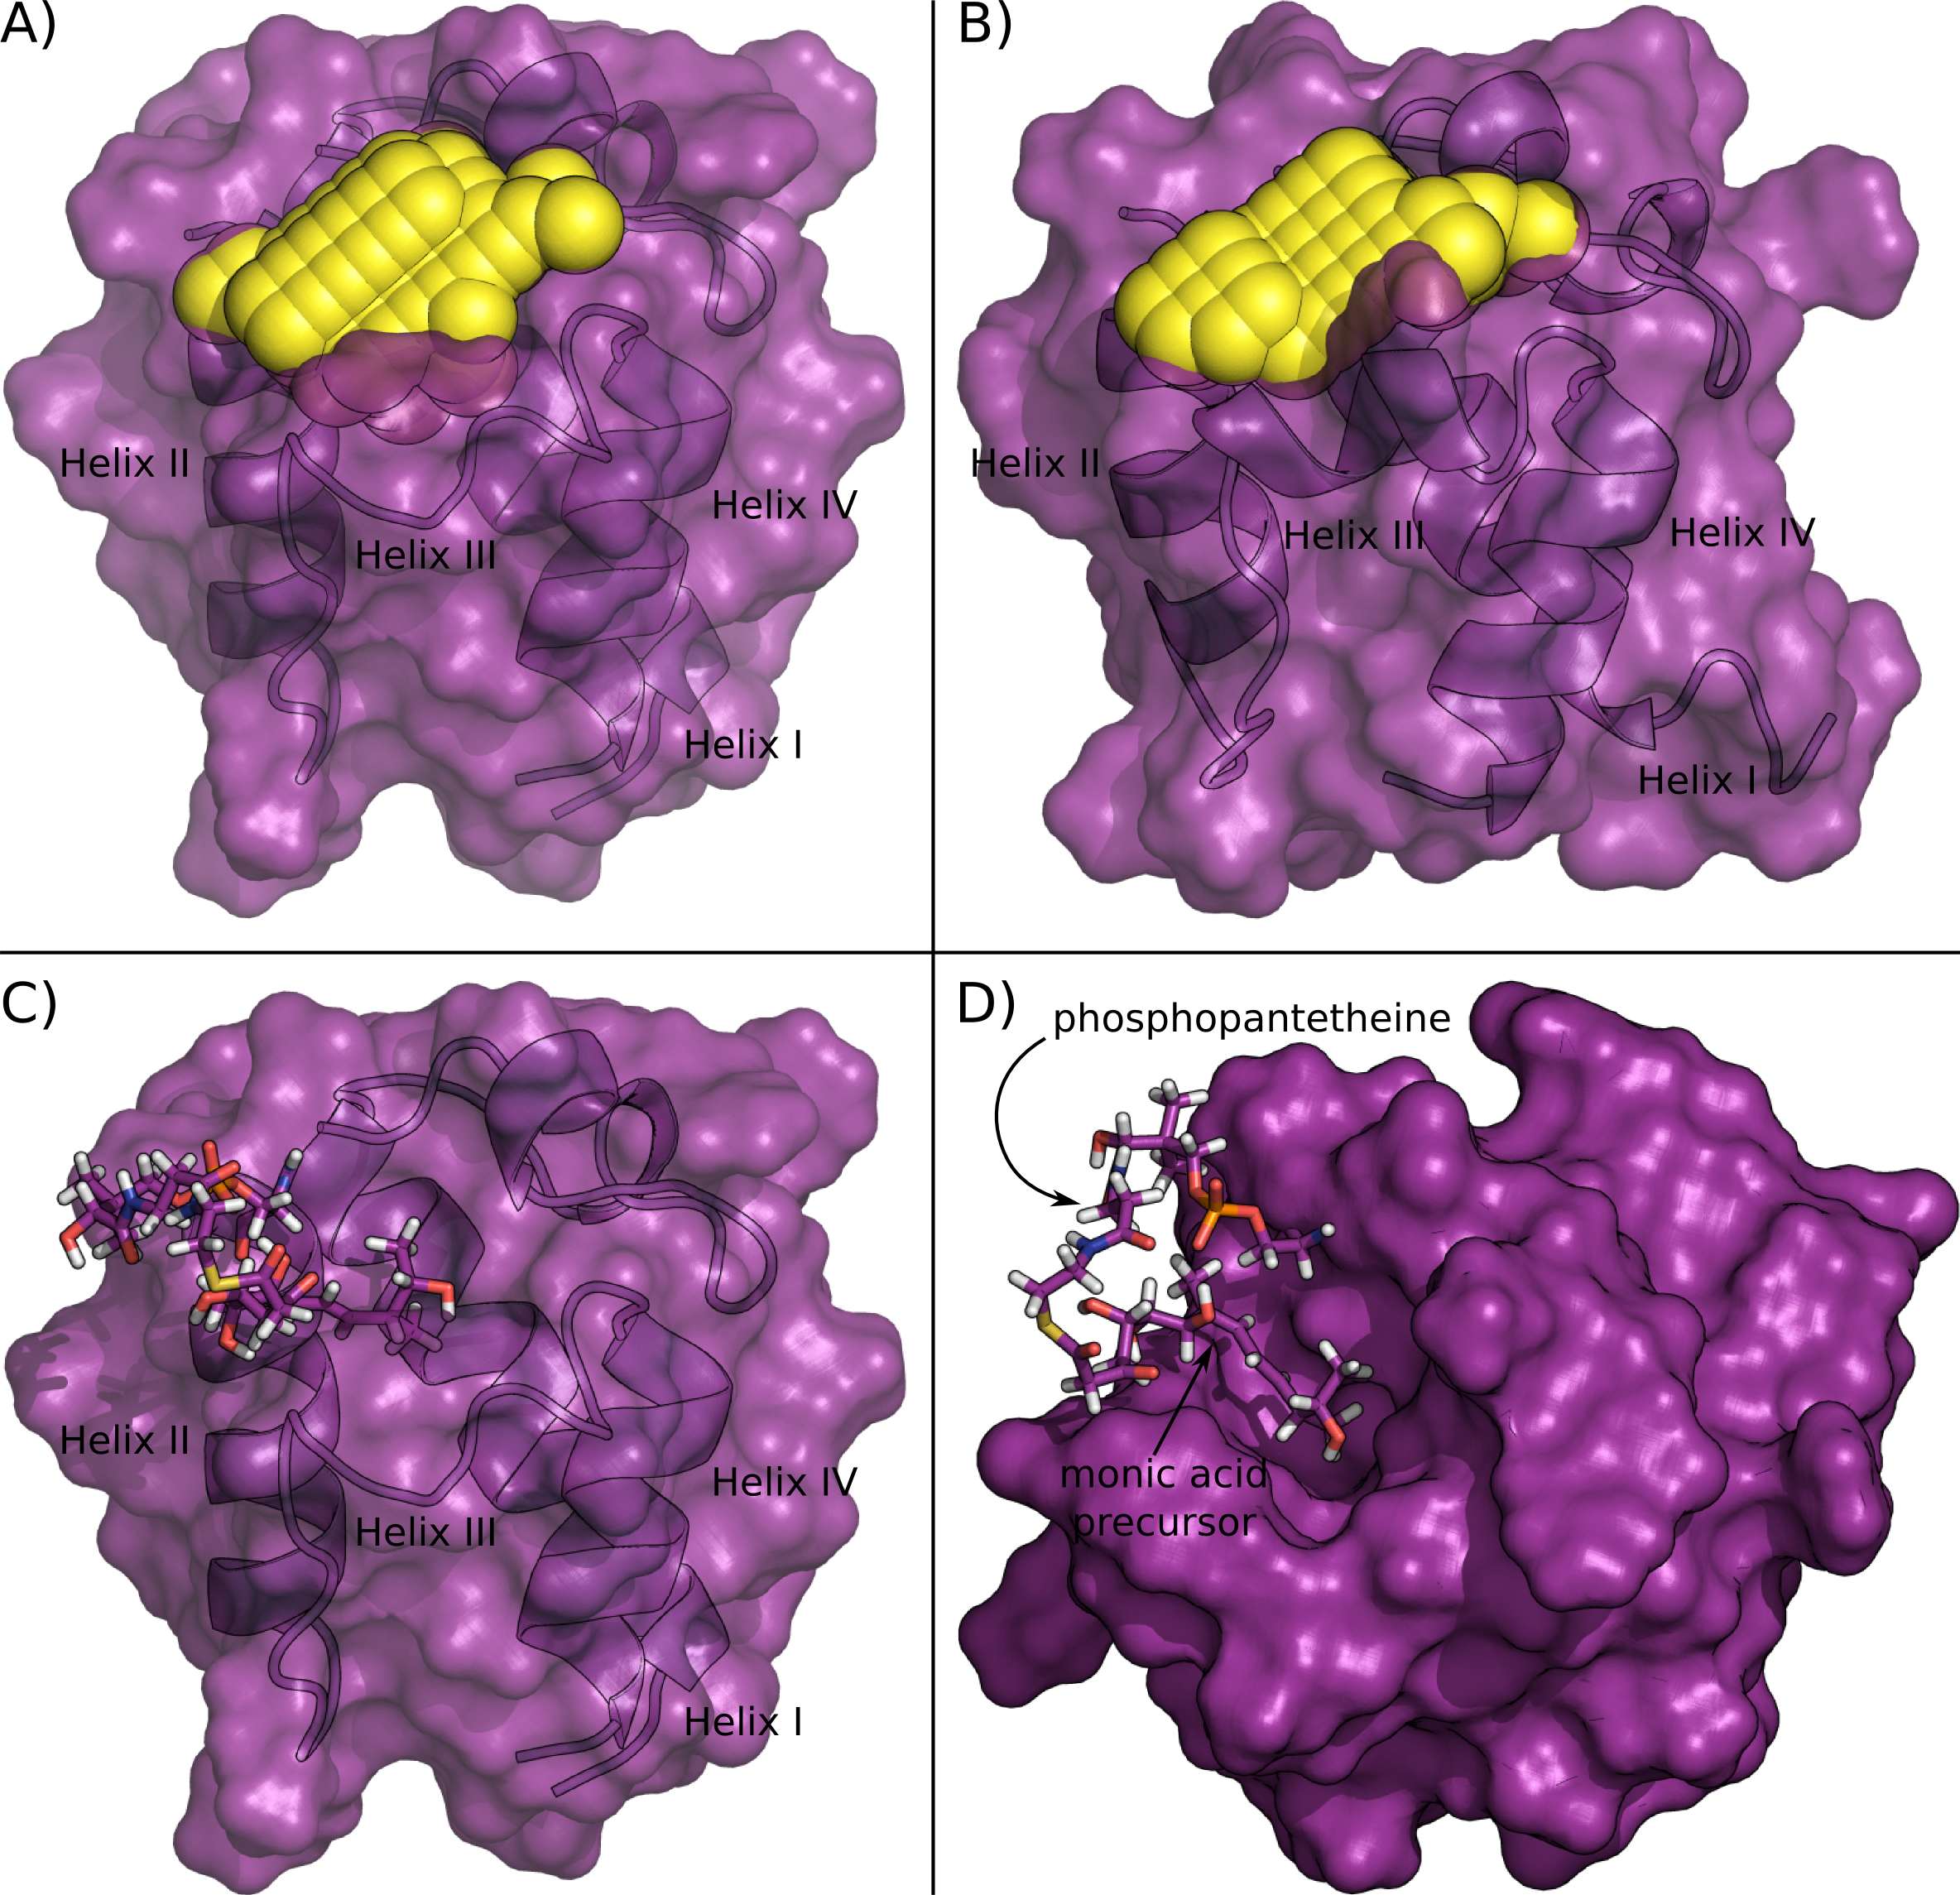
\includegraphics[width=0.9\textwidth,keepaspectratio=true]{graphics/spm_cavities.png}}
		\caption[Largest cavity detected in the acyl ACP-mupA3a WT.]{Largest cavity detected in the acyl ACP-mupA3a WT. (A \& B) space filled (yellow spheres) drawing of the largest and the modal cavity volume respectively. (C \& D) orientation of the ligand in the cavity formed in two different views.}
		\label{fig:spm_cavities}
		\end{figure}

\newpage			
	%Largest volume Table
	\begin{table}[h]
	\caption{Largest and modal cavity volume for each simulation}
	\label{tab:largestcavity}
	\begin{tabular}{p{4cm}|c c|c c}
	\toprule[2pt]
	\textbf{Simulation} & \multicolumn{ 2}{c|}{\textbf{WT}} & \multicolumn{ 2}{c}{\textbf{W44L}} \\ 
	\textbf{} & \multicolumn{1}{p{3cm}}{\textbf{Largest cavity volume}} & \multicolumn{1}{p{2cm}|}{\textbf{Modal volume}} & \multicolumn{1}{p{3cm}}{\textbf{Largest cavity volume}} & \multicolumn{1}{p{2cm}}{\textbf{Modal volume}} \\ 
	\midrule[1pt]
	Apo ACP-mupA3a (200ns) & 151.593 & 52.728 & 173.563 & 50.531 \\ 
	Apo ACP-mupA3a (1$ \mu $s) & 151.593 & 52.728 & - & - \\ 
	Holo ACP-mupA3a & 228.488 & 109.85 & 243.867 & 92.274 \\ 
	Acyl ACP-mupA3a (200ns) & 265.837 & 103.259 & 243.867 & 57.122 \\ 
	Acyl ACP-mupA3a (1$ \mu $s) & 265.837 & 72.501 & - & - \\ 
	Acyl 14C ACP-mupA3a & 195.533 & 96.668 & - & - \\ 
	Acyl ACP-mupA2a & 248.261 & 92.274 & - & - \\ 
	\bottomrule[2pt]
	\end{tabular}
	\end{table}

	
	
\newpage	
	\subsection{Change in RMSD of PKS ACPs from FAS ACP over time}
	\label{sec:rmsd}
	In watching movies of the simulations it seemed that holo and acyl forms of the PKS ACPs become more like FAS ACPs in structure. It seemed that the structure might be responding to the presence of the ligands to produce a cavity. To quantify whether there was a relationship between cavity volume and similarity to FAS structure the correlation was calculated 
	%As it was observed, that the binding of the ligand to the PKS ACPs induces the formation of the cavity, it was interesting to test whether the PKS ACPs change and become more like FAS type, in order to accommodate the ligand inside the core. 
	between the cavity volume at every ns and the RMSD of the backbone atoms of the PKS ACPs from the FAS ACP reference structure (Table \ref{tab:correlations}). A weak negative correlation was observed in all the structures except in the acyl ACP-mupA2a i.e. as the volume increases the similarity to FAS increases, albeit only slightly. The correlations were slightly stronger in the ACP-mupA3a W44L structures with the strongest in holo ACP-mupA3a W44L simulation. Comparing the Figures \ref{fig:CavityVolumeACPPTMutant_nonzero} and \ref{fig:RmsdAcpPPTMutant1} shows a high rise in the RMSD between 120 and 160 ns which strongly correlates with the sudden dip in the cavity volume in the same time frame. Figures from \ref{fig:RmsdAcpWild} to \ref{fig:RmsdACP2} in the Appendix III show the change in the RMSD of the backbone atoms of each PKS ACP from the FAS ACP over time. Taken individually these correlation coefficients might seem insignificant but the fact that they are all negative does point to a small but significant effect.
	
		\setlength\fboxsep{5pt}
		\setlength\fboxrule{1.5pt}
		\begin{figure}[htbp]
		\centering
		\fbox{\includegraphics[width=0.9\textwidth, keepaspectratio=true]{graphics/CavityVolumeACPPPTMutant_nonzero.png}}
		\caption[Formation and change in cavity volume over time in the holo ACP-mupA3a W44L.]{Formation and change in cavity volume over time in the holo ACP-mupA3a W44L. The time frames which had a zero value for the volume were omitted from the plot. Red line represents the running average over 500 frames and green line represents the mean.}
		\label{fig:CavityVolumeACPPTMutant_nonzero}
		\end{figure}	
		
		\setlength\fboxsep{5pt}
		\setlength\fboxrule{1.5pt}
		\begin{figure}[htbp]
		\centering
		\fbox{\includegraphics[width=0.9\textwidth, keepaspectratio=true]{graphics/RmsdAcpPPTMutant.png}}
		\caption[RMSD between FAS ACP and the holo ACP-mupA3a W44L over time.]{RMSD between FAS ACP and the holo ACP-mupA3a W44L over time. Green line represents the mean.}
		\label{fig:RmsdAcpPPTMutant1}
		\end{figure}	
	
	\subsection{Hydrogen bonding between the phosphopantetheine, acyl groups and protein/solvent}
	\label{sec:hb}
	In watching movies of the simulations, the phosphopantetheine and acyl chains were seen to interact with the protein. However, as the cavity detected during the simulation was shallow and solvent exposed the ligands seemed to be in partial interaction with the solvent as well. To detect the interaction of the ligands with the protein and solvent hydrogen bonds were measured between the ligands and the protein/solvent throughout the simulation. Table \ref{tab:averages} shows the mean number of hydrogen bonds per frame formed with the protein and solvent (columns 3 and 4 respectively) by the phosphopantetheine and the acyl groups. It was observed that the phosphopantetheine constantly makes hydrogen bonds with the solvent, with a very slight drop in the average number when an acyl group is attached, as compared to without substrate. No significant correlation was found between the cavity volume and the hydrogen bonds formed between the ligand and the protein. However, a negative correlation was observed between the hydrogen bonds formed by the ligand with the protein and the solvent. This negative correlation showed a general trend of a rise of hydrogen bonds made by the ligand with the protein and fall of hydrogen bonds made by the ligand with the solvent over time (see Figures from \ref{fig:HbondACPPPTWild_protein} to \ref{fig:HbondACP2_solvent} in Appendix III). A general trend where for every hydrogen bond formed between ligand and protein one between ligand an solvent is lost would be expected.

	
	%Correlation table
	\begin{sidewaystable}[htbp]
	\caption{Correlation between cavity volume and RMSD / hydrogen bonds. }
	\label{tab:correlations}
	\begin{small}
	\begin{tabular}{l|cc|cc|cc}
	\toprule[2pt]
	\multicolumn{1}{p{5cm}|}{\textbf{Simulation}} & \multicolumn{ 2}{p{5cm}|}{\textbf{Correlation between cavity volume and RMSD from the FAS ACP}} & \multicolumn{ 2}{p{5cm}|}{\textbf{Correlation between cavity volume and hydrogen bonds with the protein}} & \multicolumn{ 2}{p{5cm}}{\textbf{Correlation between the hydrogen bonds formed by the ligand with protein and solvent}} \\ 
	\textbf{} & \textbf{Wild} & \textbf{W44L} & \textbf{Wild} & \textbf{W44L} & \textbf{Wild} & \textbf{W44L} \\ 
	 &  &  &  &  &  &  \\ 
	 \midrule[1pt]
	\multicolumn{1}{p{5cm}|}{Apo ACP-mupA3a (200ns)} & -0.241 & -0.309 & - & - & - & - \\ 
	\multicolumn{1}{p{5cm}|}{Apo ACP-mupA3a (1$ \mu $s)} & -0.241 & - & - & - & - & - \\ 
	\multicolumn{1}{p{5cm}|}{Holo ACP-mupA3a} & -0.225 & -0.601 & 0.041 & 0.021 & -0.433 & -0.222 \\ 
	\multicolumn{1}{p{5cm}|}{Acyl ACP-mupA3a (200ns)} & -0.111 & -0.435 & 0.164 & 0.015 & -0.653 & -0.323 \\ 
	\multicolumn{1}{p{5cm}|}{Acyl ACP-mupA3a (1$ \mu $s)} & -0.245 & - & 0.203 & - & -0.429 & - \\ 
	\multicolumn{1}{p{5cm}|}{Acyl 14C ACP-mupA3a} & -0.538 & - & - & - & - & - \\ 
	\multicolumn{1}{p{5cm}|}{Acyl ACP-muA2a} & 0.143 & - & 0.012 & - & -0.207 & - \\ 
	\bottomrule[2pt]
	\end{tabular}
	\end{small}

	\end{sidewaystable}
	
	\subsection{Structural and sequence comparison of the \textit{E. coli} FAS ACP and ACP-mupA3a}
	\label{sec:PKSFASACP}
	In order to understand what might be preventing ACP-mupA3a from forming a deep tunnel shaped cavity, FAS ACP (PB ID 1L0I) and ACP-mupA3a structures were compared by structural and sequence alignments. Figure \ref{fig:pks_fas_comp} shows the superimposed structures of the reference FAS ACP (PDB ID 1L0I) and apo ACP-mupA3a WT. Two noticeable differences in the residue positions were observed which might be associated (amongst others) with the tunnel shaped cavity found in the FAS ACPs. Residue 59 on helix III of the FAS ACP is an alanine, but is equivalent to I61 in the ACP-mupA3a. In Figure \ref{fig:pks_fas_comp} (B) the bulky isoleucine can be seen as a hindrance in the path leading to the deep tunnel. Similarly A34 in the FAS ACP is equivalent to L36 in ACP-mupA3a, this position corresponds to the residue between G and D in the GXDS motif and is usually a bulky residue in PKS ACPs.
	
		\setlength\fboxsep{5pt}
		\setlength\fboxrule{1.5pt}
		\begin{figure}[htbp]
		\centering
		\fbox{\includegraphics[width=0.9\textwidth, keepaspectratio=true]{graphics/pks_fas_comp.png}}
		\caption[Structural comparison of an FAS ACP (PDB ID 1L0I) and an apo ACP-mupA3a WT.]{Structural comparison of an FAS ACP (PDB ID 1L0I; green) and an apo ACP-mupA3a WT (cyan). (A) positions A59/I61, L42/W44 and a butyryl molecule attached to the phosphopantetheine in the FAS ACP are drawn as sticks and position A34/L36 as lines. (B) surface drawing of the FAS ACP (green) highlighting the orientation of the ligand and opening of the tunnel shaped cavity I61 (cyan sticks) can be seen as a blockage in the tunnel.}
		\label{fig:pks_fas_comp}
		\end{figure}	
	
	In order to understand the sequence conservation of these positions in the FAS and PKS ACPs two sets of similarity searches were carried out using PHI BLAST against the NCBI's non redundant protein database. The first search used the sequence of FAS ACP (PDB ID 1L0I) as the query along with the motif GADS, a highly conserved motif in the FAS ACPs. This search matched 1055 unique sequences with 95\% query coverage or greater (sequences with large insertions were removed from the alignment). These 1055 unique sequences represented species from 473 genera with an average sequence identity of 65\%.  Figure \ref{fig:gads_95} shows the sequence logo built on the multiple sequence alignment of the 1055 unique FAS ACP sequences. A59 of helix III was found to be absolutely conserved in all the sequences, along with the two highly conserved glutamic acid residues immediately before and one highly conserved glutamic acid residue immediately after position 59 (i.e. an EEAE motif). Searching the FAS ACP sequence against the NCBI's non redundant protein database with the EEAE motif yielded 472 unique sequences with at least 95\% query coverage. Figure \ref{fig:eeae_95} shows the sequence logo built using the multiple sequence alignment of the 472 unique FAS ACP sequences with the EEAE motif. It was interesting to observe that by searching with the GADS motif A59 was found absolutely conserved and while searching with the EEAE motif A34 was found absolutely conserved as well. Comparing the two sequence logos one can say that the FAS ACPs are highly conserved with an average sequence identity of 65\% and 76\% when searched with the GADS and EEAE motifs respectively. The FAS ACP sequence was also searched against the PDB database with the GADS and EEAE motifs, which matched 11 and 8 FAS ACP structures respectively with the similar sequence conservation pattern as shown in sequence logos in Figures \ref{fig:gads_95} and \ref{fig:eeae_95}. 

		\setlength\fboxsep{5pt}
		\setlength\fboxrule{1.5pt}
		\begin{figure}[htbp]
		\centering
		\fbox{\includegraphics[width=\textwidth, keepaspectratio=true]{graphics/gads_95.png}}
		\caption[Sequence logo built on 1055 unique FAS ACP sequences containing a GADS motif.]{Sequence logo built on 1055 unique FAS ACP sequences containing a GADS motif (position 34-36).}
		\label{fig:gads_95}
		\end{figure}	

		\setlength\fboxsep{5pt}
		\setlength\fboxrule{1.5pt}
		\begin{figure}[htbp]
		\centering
		\fbox{\includegraphics[width=\textwidth, keepaspectratio=true]{graphics/eeae_95.png}}
		\caption[Sequence logo built on 472 unique FAS ACP sequences containing a EEAE motif.]{Sequence logo built on 472 unique FAS ACP sequences containing a EEAE motif (position 57-60).}
		\label{fig:eeae_95}
		\end{figure}			
	
	Searching with the \textit{E. coli} FAS ACP sequence (PDB ID 1L0I) without any additional motif constraint against NCBI's non redundant protein database matched 2078 unique sequences with 95\% or greater query coverage. Alignment of these sequences revealed three broad groups: group one contains the GADS motif (1280 sequences), group two contains a GLDS motif instead of the GADS motif (257 sequences) and group three has neither a GADS or a GLDS motif (541 sequences). The third group also lacked the conservation of G in the GXDS motif. Figures from \ref{fig:gadsnopattern} to \ref{fig:neithersnopattern} in Appendix III show the sequence logos built on the above mentioned three sets of sequences. The sequences which carry a GADS motif show a high conservation of alanine at the 59th position of the FAS ACP structure. The sequences which carry a GLDS motif have a position 59 with predominantly A, L and R but also other residues. The alignment/logo of FAS ACP sequences which did  not carry either of these motifs indicates poor conservation at most of the positions. 
	
	FAS ACP sequences carrying a GLDS motif are more like PKS ACPs with a bulky residue	at the X position in the GXDS motif and another bulky reside at the equivalent position of I61 in ACP-mupA3a, equivalent to A59 in the FAS ACP structure discussed in the previous paragraph. Figures \ref{fig:branchingacplogo} and \ref{fig:standardacplogo} show the sequence logos built on the ACPs from 15 well characterised PKS clusters grouped into ACPs associated with \bet-branching and standard ACPs as used in Chapter \ref{cha:ACP-HCS}. Both the sequence logos show the presence of a bulky residue at the X position in the GXDS motif, which co-occurs with the bulky reside at the equivalent position of I61 (ACP-mupA3a). These observations suggest that having a less bulky residue at the position A59/I61 is correlated with a sequence being an FAS ACP and presumably allows the formation of a deep tunnel shaped cavity in the FAS ACPs. Owing to a high level of sequence conservation in the FAS ACPs this structural feature would be shared widely. 
	
		\setlength\fboxsep{5pt}
		\setlength\fboxrule{1.5pt}
		\begin{figure}[htbp]
		\centering
		\fbox{\includegraphics[width=\textwidth, keepaspectratio=true]{graphics/branchingacplogo.png}}
		\caption[Sequence logo built on the \bet-branching ACP sequences from 15 well characterized polyketide synthase clusters.]{Sequence l ogo built on the \bet-branching ACP sequences from 15 well characterized polyketide synthase clusters. \textcolor{red}{- - - - -} indicates the GXDS position and \textcolor{red}{*} indicates the position 55 equivalent to A59 in the FAS ACPs or I61 in MupA.}
		\label{fig:branchingacplogo}
		\end{figure}			
		
		\setlength\fboxsep{5pt}
		\setlength\fboxrule{1.5pt}
		\begin{figure}[htbp]
		\centering
		\fbox{\includegraphics[width=\textwidth, keepaspectratio=true]{graphics/standardacplogo.png}}
		\caption[Sequence logo built on the standard ACP sequences from 15 well characterized polyketide synthase clusters.]{Sequence logo built on the standard ACP sequences from 15 well characterized polyketide synthase clusters. \textcolor{red}{- - - - -} indicates the GXDS position and \textcolor{red}{*} indicates the position 55 equivalent to A59 in the FAS ACPs.}
		\label{fig:standardacplogo}
		\end{figure}			

\newpage					
\section{Discussion}
\label{sec:chap5discussion}
In order to investigate the possible formation of a cavity and the sequestering of phosphopantetheine and acyl chains in the ACP core, a series of molecular dynamics simulations were performed on the apo, holo and acyl forms of the ACPs from the MmpA module of the mupirocin cluster (ACP-mupA3a and ACP-mupA2a). Experimentally determined ACP structures and molecular dynamics studies on FAS ACPs have shown the formation of a hydrophobic tunnel within the ACP core, which sequesters the growing saturated fatty acid chain, protecting it from the outer hydrophilic environment, but this had not been seen for PKS ACPs. \textcite{Chan2008} have shown that an optimal acyl chain length from eight carbons up to ten carbons can be stably accommodated by the \textit{E. coli} FAS ACP. In this chapter, the acyl chains were of 12C and 14C backbone atoms long. Three independent simulations of 50 ns each were set up for all the structures namely apo ACP-mupA3a (WT and W44L), holo ACP-mupA3a (WT and W44L), acyl ACP-mupA3a (WT and W44L), acyl 14C ACP-mupA3a and acyl ACP-mupA2 were setup. The starting structures for the holo as well as the acyl structures had solvent exposed ligands attached to the catalytic serine. \textcite{Chan2008} ran 50 ns simulations for the structures with solvent exposed acyl chains, the time scale was enough for acyl chains of four, six, eight, ten and sixteen carbons in length to find their way into the cavity. Acyl chains with twelve, fourteen and eighteen carbons failed to find the cavity even in extended simulations. 

Here, three independent 50 ns simulations per holo and acyl structure seem to be a good starting point for sampling enough phase space for the ligands to find their way into the proposed cavity. However, as there was no experimental evidence of cavity formation and sequestering of acyl chains in the PKS systems, there was no clear idea of how long a simulation should be to see the sequestering of the ligand, if indeed sequestering occurred. Therefore, one of the multiple 50 ns simulations that showed a transition of the acyl chain into the proposed cavity space was extended upto 200 ns for apo and holo ACPs, with one simulation of the wild type ACP-mupA3a charged with its cognate substrate simulated for 1$ \mu $s. The simulation of the apo ACP-mupA3a WT was also extended to 1 $ \mu $s as a control.

The root mean square deviation (RMSD) of the backbone atoms of the simulated structures from their reference starting structure remained under 2.5 \AA, suggesting that the structures in apo, holo or acyl forms did not undergo any extreme unfolding events. This observation was crucial to test the stability of the holo and acyl forms since the solved ACP-mupA3a structure did not have the coordinates for the phosphopantetheine or for any of the acyl chains. The topology information for the phosphopantetheine and the acyl chains were built manually and the bond, angle, dihedral and van der Waals forcefield parameters were derived from the General Amber Force Field (GAFF), with partial charges  derived by the RESP method, since these parameters were not in the GROMACS suite. The GAFF parameters and RESP charges were designed to be compatible with the AMBER99SB-ILDN forcefield.

\textcite{Chan2008} utilized the GROMOS96 43a2 forcefield for their ACP simulation and most of the atom types in the acyl chain and parameters for the for the atom types which were not present in the parent GROMOS96 43a2 forcefield database were generated through GAUSSIAN quantum mechanics software. Observations from their simulations were similar to what was observed here. RMSF values showed a general trend of more fluctuation in the mutant structures as compared to their wild type counter parts, these observations are consistent with the MD simulations mentioned in Chapter 3, Section \ref{sec:WtoLMD}. Most of the fluctuation was observed from residues 34 to 40 (around the catalytic S38) and 52 to 68 (loop II and helix III).

A cavity was detected in more time frames during the holo and ACP simulations as compared to the apo ACP-mupA3a structures. The cavity volumes detected for the holo as well as the acyl forms were also larger in size as compared to the apo structures. These observations suggested that the attachment of phosphopantetheine and acyl chains not only induced the formation of the cavity but that the attachment also influenced the size of the cavity formed. Upon utilizing the same parameters for the cavity detection the reference FAS ACP (PDB ID 1L0I) structure recorded a volume of 253 \AA$ ^{3} $ which was comparable to the largest cavity detected for acyl ACP-mupA3a WT. However, the shape of the cavity for the FAS ACP was found to be like a deep tunnel as compared to the wide, shallow and surface exposed cavity in the PKS ACPs. A similar trend for wide, shallow and surface exposed cavities, as those seen in the ACP-mupA3a WT was seen in the other simulations of PKS ACPs performed here. 

\textcite{Chan2008} found that the average cavity volume continuously increases in size according to the size of the ligand for upto ten carbons and but for chains between 10 and 18 carbon long remained unchanged. Here the acyl chains are twelve and fourteen backbone carbons long and the cavity volumes seen in these simulations do not seem to vary with chain length. Interestingly the average size of the cavity induced by the phosphopantetheine alone was also of the same size as that induced by the fourteen backbone carbon long acyl form. Visual inspection of the MD simulation trajectory revealed that the phosphopantetheine occupies the same cavity space as the substrate occupies in the acyl ACP-mupA3a simulations, in the latter case the phosphopantetheine is in solvent. This observation may be because the size of the phosphopantetheine backbone is similar to the size of the ACP-mupA3a cognate substrate backbone (i.e. 14C). and because the shape of the cavity is surface exposed the highly polar phosphopantetheine can hydrogen bond with the solvent while still residing in the cavity.

The shallow surface exposed cavities also meant that no part of the acyl chains was buried inside the ACP but rather the acyl chains were in constant interaction with the solvent. This hypothesis was based on the thinking that the polyketide molecules usually have some polar groups which can hydrogen bond with the solvent and do not necessarily require a hydrophobic casing to segregate them from the solvent. This does not equally apply to the FAS ACPs because the acyl chains in fatty acid synthesis are usually saturated and non polar in nature (except the \bet-carbon processed intermediates) and would experience a constant repulsion from the solvent. It would rather be energetically favourable for a highly hydrophobic chain to envelope itself within a hydrophobic core. In principle a hydrophobic chain without such sequestration inside the ACP, could also attach itself to other hydrophobic entities in the cell making it not available to the FAS proteins. 

The hypothesis that the acyl chains were in constant interaction with the solvent was also supported by the observation that the SASA calculated for the phosphopantetheine and the acyl chains (once the ligands have associated themselves with the protein)  over time was constant,  avoiding any further dips which would have suggested a transition from a less to more buried state. \textcite{Chan2008} showed a very low solvent accessible surface area (SASA) for the acyl chains upto eight carbons long, which increases rapidly for an acyl chain of ten to eighteen carbons long, as the FAS ACP could not shield completely a carbon chain more than ten carbons long. The lowest SASA value recorded for an acyl chain in the PKS ACPs was for acyl 14C ACP-mupA3a, which was $ \approx $43 \AA$ ^{2} $, $ \approx $9.5 \AA$ ^{2} $ more than the SASA value calculated for the 14C acyl chain by \textcite{Chan2008}. Not surprisingly the highest SASA value calculated was for the phosphopantetheine, which was $ \approx $16 \AA$ ^{2} $ more than the SASA for the 14C saturated acyl chain. The SASA calculations were also supported by the number of hydrogen bonds made between the ligands (phosphopantetheine and the acyl chains) and the protein/solvent. Phosphopantetheine as well as the acyl chains were constantly making hydrogen bonds with the solvent as well as the protein, although the number of H-bond to solvent did not correlate with the size of the cavity induced. 

During the smulations, as the PKS ACPs become more like the FAS ACP structure the volume of the cavity increased, as evidenced by the RMSD between the PKS and FAS ACPs decreasing as the cavity volume increased (negative correlation) in all the structures except one. %The idea behind calculating a correlation between the two was, to test whether the PKS ACP fold draw towards the FAS ACP fold, while enveloping the phosphopantetheine or acyl chains. A negative correlation between the cavity volume and the backbone atom RMSD of the PKS ACPs from FAS ACP suggests that the PKS ACPs backbone was drawing closer to the FAS ACP reference structure. 
However, as the cavity formed in the PKS structures is wide, shallow and surface exposed, as compared to deep tunnel in the FAS ACP, it is clear that only part of the structure was changing to be like an FAS ACP. A stronger correlation between the FAS and W44L mutant ACP structures suggested that having a less bulky residue in the PKS ACP core might allow the PKS ACPs structures to move closer to the reference FAS ACP. 

Comparing the PKS apo ACP-mupA3a WT structure with the reference FAS ACP, revealed I61 in the ACP-mupA3a (which is an A59 in the FAS ACP) blocking the entry of the tunnel. Multiple sequence alignment of FAS and PKS ACPs revealed that position I61/A59 is highly conserved with an alanine in the FAS ACP and a bulkier residue in the PKS ACPs. This position also seems to have co-evolved with the X of the GXDS motif (active site serine) in the PKS and FAS ACPs, with a bulky residue at the position X in the PKS ACPs and an alanine in the FAS ACPs. It would be interesting to mutate position I61 and/or X in the GXDS motif to alanine in the ACP-mupA3a and possibly monitor a deeper transition of the acyl chain through NMR.

The observations here support the hypothesis that the PKS ACPs do form a cavity upon the attachment of the phosphopantetheine and acyl chains. However, whether different chain lengths influence the size of the cavity was not tested. %The length of the acyl chain might also influence the size of the cavity however, as the length of the acyl chain here were of similar sizes therefore it was difficult to distinguish between them. 
The cavity formed does not form a deep tunnel that envelopes the acyl chain and thus shields it from the solvent, but is solvent exposed which enables the polar groups on the acyl chain to hydrogen bond with the solvent. It was also seen that I61 in the PKS ACPs is bulkier than A59 in the FAS ACPs and prohibits the formation of a deep tunnel. In the absence of any experimental data in this regard another set of MD simulations in a different PKS system for example ACP from module 2 of DEBS system (PDB ID 2JU1) and ACP from curacin system (PDB ID 2LIU) could be performed to verify a similar mechanism of acyl chain sequestering as observed here. It would also be interesting to test whether an FAS ACP would envelope a polyketide molecule into its  hydrophobic core in lieu of a fatty acid acyl chain. These studies might explain the dynamic mechanism through which small proteins like an ACP recognize/interact with various domains in a complex PKS machinery. The information gathered from such studies not only helps to gain a deeper understanding of protein structure and function in general but would also help to re-engineer PKS pathways for the production of novel compounds. 